
\section{Log structured merge tree (LSM)\index{LSM}}

After having finished our implementation, we wanted to compare it with another one in order to have a comparison on which to base ourselves and to note or not the interest of such a structure. We looked for a comparable data structure that offers the same features as a dictionary\index{Dictionnary} and that exists on the GPU\index{Graphics cards}. The choice was not long to decide since there is only one other offering these operations. There are works on Bounding Volume Hierarchy or R-trees but beyond the hash tables\index{Hash table}, it is somewhat lean cow. There are very few data structures specifically designed for such devices.

The Log Structured Merge tree (which we will name later LSM\index{LSM}) is a dynamic dictionary\index{Dictionnary} data structure for the GPU\index{Graphics cards}. It was developed at the end of 2017 by S. Ashkiani, S. Li, M. Farach-Colton, N. and J. D. Owens as part of a doctoral thesis of the main author~\cite{ashkiani2017parallel}. It aims to address three issues. First, it is very difficult to maintain a data structure in a dynamic context, some of the literature is devoted to creating static structure~\cite{alcantara2011building, popov2007stackless}, so a total reconstruction is re-done each time; here, updating the structure remains competitive. Second, it aims to propose operations related to dictionaries\index{Dictionnary}, namely the canonical ones: insertion/deletion/look up as well as range and count which can be seen as predecessor queries if we omit one bound. Third, exploit the capabilities of the graphics card\index{Graphics cards} while ensuring the correctness of the structure. The invariant proposed by this data structure is very strong.

This data structure is the result of the fusion of two concepts: the Log-structured Merge-tree (LSM)\index{LSM}~\cite{o1996log} and the Cache Oblivious Lookahead Array (COLA)\index{Cache oblivious}~\cite{bender2007cache}. The basic idea of a LSM\index{LSM} is to contain a set of dictionaries\index{Dictionnary} of increasing size. The elements are inserted in the first dictionary\index{Dictionnary} and when it is complete, its content is merged with the next one in the list and so on. This has two consequences, to search for an element, you have to look in each dictionary\index{Dictionnary}, which induces a cost of $O(\log N \log_{B} N)$, but to insert elements, you benefit more from the locality of the data since you merge two adjoining levels. In practice, the insertions are faster than for a B-Tree but the queries are slower. COLA, on the other hand, consists simply in having an array sorted instead of dictionaries\index{Dictionnary}.

The best way to exploit the parallelism offered by graphics cards\index{Graphics cards} for such a data structure is to work by batch. We therefore set a parameter $b$ which corresponds to the number of elements we want to insert at each step and which is equal to the size of the first buffer in this structure. Both update operations are performed by batch, insertions and deletions. Queries do not depend on this parameter and can be performed by a single thread.

\begin{figure}[!htb]
    \centering
    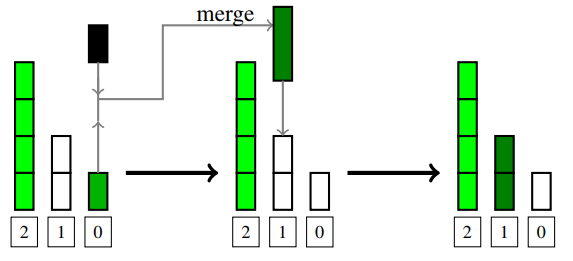
\includegraphics[width=0.75\linewidth]{Chapters/ParallelXFastTries/LSM.png} 
    \caption{Batch insertion with already 5 inserted batches - image extracted from Ashkiani et al.~\cite{ashkiani2017gpu}, arXiv:1707.05354}
\end{figure}

Let's first clarify that the different dictionaries\index{Dictionnary} used internally by this data structure have sizes that are powers of 2 and multiples of $b$ (i.e. $b2^{i}$). To insert or delete elements, we first sort the data related to the batch. Then, we always apply the same procedure, we check if the $i$th level is complete or empty (they cannot be partially filled), if it is empty, we insert all our elements. Otherwise, the elements to be inserted are merged with the elements of the $i$th level, the two containers become one and the previously filled level is emptied. We then try to insert the result in the next container, and so on until we find an empty dictionary\index{Dictionnary}. It should be noted that the filled levels correspond to the bit set to 1 in the binary representation of the number of batches inserted $r$, and 0 for the empty ones. There are thus $n = br$ elements in the structure. The total amount of work to insert $n$ elements is thus $O(rb \log r)$ since the worst case is complete cascading $O(rb)$ and this occurs with $O(i) \leq O(\log r)$. Observe that duplicates may exist naturally and that deletions correspond to sentinel values sharing the same key. In their implementation, they propose to set the most significant bit to 1 to indicate a deletion, which will serve in the merge procedure.

Queries can be simply implemented through classic lower/upper bound queries on each filled level and leading to natural $O(\log^{2} n)$. Note that merge procedures are somewhat difficult to implement in a parallel context, especially when duplicates exist~\cite{green2012gpu}.